\chapter{Угадыватель чисел}
\label{ch:guessnumbers}

В этой главе мы познакомим вас с программой «Угадыватель чисел»~\cite{PanfilovaApp}, идея которой взята из книги Л. Ф. Магницкого, «Арифметика»~\cite{Galanin}. 
Опишем задачу и расскажем как запрограммировать решение. Поработаем с экранами приложения, создадим процедуры и покажем как разрешить ввод только числовых значений в программе.


\section{Описание задачи}

Суть предлагаемой нами задачи описана в книге Л. Ф. Магницкого «Арифметика», в главе: «Об утешных некиих действиях, через арифметику употребляемыx»~\cite{Galanin}.

Пронумеруем дни недели от одного (понедельник) до семи (воскресенье). 
Предложим игроку загадать число, равное номеру любого дня недели. Далее попросим загадавшего выполнить следующие действия:
\begin{enumerate}
\item Умножить номер загаданного дня недели на два.
\item К полученному произведению прибавить пять.
\item Затем полученную сумму умножить на пять.
\item Полученное число умножить на десять.
\item Назвать результат вычислений.
\end{enumerate}

Таким образом, с помощью этих арифметических преобразований мы легко сможем определить, какое число загадал игрок.

\section{Решение задачи}

Раскроем секрет математического фокуса. Чтобы перейти от полученного числа к загаданному, необходимо вычесть из него двести пятьдесят и поделить полученное число на сто. Таким образом, мы получим число, в котором номер дня недели – число сотен в числе. Рассмотрим доказательство решения задачи. Пусть $ a $ — искомое число (день недели). Выполним указанные действия над числом $ a $:

\begin{enumerate}
   \item $2\cdot a $

   \item $2\cdot a + 5$

   \item $5\cdot(2 \cdot a  + 5) = 10 a + 25$
 
   \item $(10a + 25)\cdot 10 = 100  a + 250$
 
   \item  $\frac{100  a + 250 - 250}{100} =  a $
\end{enumerate}

Доказательство выполнено, и мы получили число $  a $.

\begin{mdfstyle}[nobreak=true,frametitle=Вопрос]
  \sloppy   
  В доказательстве алгоритма говорится, что ($  a $ — это искомое число, но не уточняется, какое это число. Определите вид числа и его допустимые значения, приведите примеры.  Ответ на странице ... todo.
  \label{question:text}
\end{mdfstyle}

\section{Реализация приложения}
\label{styles}
В программе «Угадыватель чисел» (The Numbers Guessing Game)~\cite{PanfilovaApp} загаданный игроком номер дня недели — это то, что мы будем искать.
Создадим глобальную переменную  \textit{secretNumber} для хранения искомого числа, загаданного игроком. Присвоим этой переменной значение, равное нулю. Так как оно не входит в интервал от одного до семи, переменная  не равна загаданному числу a. Также
отметим, что в этом приложении  объекты именуются в стиле СamelCase\footnote[][-0cm]{\index{Процедуры и переменные!Именование} \emph{Именовать объекты} 
можно также произвольно, но рекомендуется использовать один из общепринятых стилей.
}\marginnote[0.2cm]{
Список самых распространённых стилей см. на с.~\pageref{answer:naming}.
}. 
\subsection{Определение числа, загаданного игроком}
Чтобы в (\textit{numberText}) пользователь мог вводить только числовые значения, необходимо поставить галочку у свойства \textit{(NumbersOnly}. Рассмотрим блок обработки нажатия (см. рис.~\ref{fig:block:button:click}) на кнопку «Узнать ответ» (Button1).
Когда игрок нажимает на эту кнопку, последовательно выполняются следующие действия:
\begin{enumerate}
  \item Вызываетcя процедура \textbf{visibleFalseImages} (рис. ~\ref{fig:block:visible:false:images}), которая устанавливает свойство Visible у всех изображений с цифрами в false. Таким образом, пока не будет определено число загаданное пользователем, изображения с цифрами не будут отображаться.
  \begin{figure}
    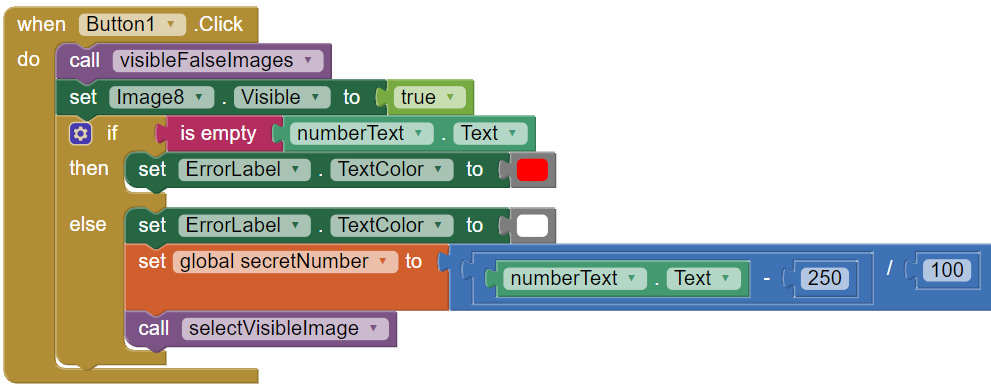
\includegraphics{./graphics/programs/guess_numbers/block_Button1Click_AppInventor_2018.png}
      \caption[Блок обработки нажатия на кнопку Button1.][6pt]{Блок обработки нажатия на кнопку Button1}
    \label{fig:block:button:click}
  \end{figure}

  \item Вызываетcя процедура \textbf{visibleFalseImages} (рис. ~\ref{fig:block:visible:false:images}), которая устанавливает свойство Visible у всех изображений с цифрами в false. Таким образом, пока не будет определено число загаданное пользователем, изображения с цифрами не будут отображаться.
  \begin{figure}
    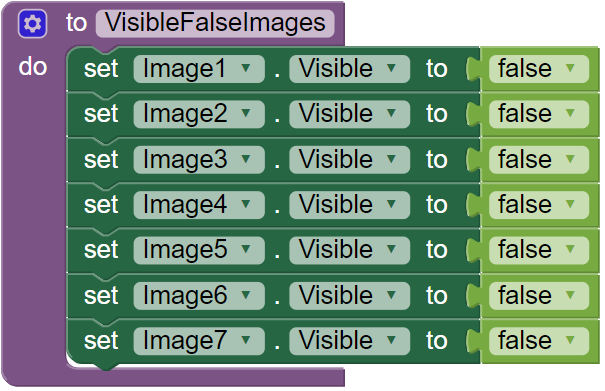
\includegraphics{./graphics/programs/guess_numbers/procedure_visibleFalseImages_AppInventor_2018.png}
      \caption[Процедура visibleFalseImages.][6pt]{Процедура visibleFalseImages устанавливает свойство Visible у всех изображений с цифрами в false.}
    \label{fig:block:visible:false:images}
  \end{figure}

  \item Устанавливается свойство \textit{Видимость} (\textit{Visible}) в значение true у изображения со знаком вопроса (Image8).
  \item Если значение поля для ввода загаданного числа (numberText) пусто, то приложение сигнализирует пользователю об ошибке следующим образом. Устанавливаем красный цвет шрифта, чтобы стало видно сообщение у поля  «Пожалуйста, введите полученное число.» ErrorLabel. В случае, когда что либо введено в поле \textit{numberText}, последовательно выполняются следующие шаги:
  \begin{itemize}
    \item Устанавливается белый цвет шрифта у поля \textit{ErrorLabel}.
    \item Производится подсчёт значения переменной \textit{secretNumber}:
    \item Вызывается процедура \textbf{selectVisibleImage}, которая будет рассмотрена далее.
  \end{itemize}
\end{enumerate}
Возникает вопрос: почему для того, чтобы отображать сообщение об ошибке мы меняем цвет текста у поля \textit{ErrorLabel}, а не управляем значением свойства \textit{Видимость} (\textit{Visible})? Дело в том, что при использовании свойства \textit{Visible} любое изменение его значения вызывает перерисовку экрана, а элементы интерфейса будут менять свои позиции, то есть скакать по экрану. В нашем приложении, если цвет поля белый, то компонент \textit{ErrorLabel} сливается с фоном экрана, сообщение об ошибке не видно.
\section{Процедура selectVisibleImage}

\begin{figure}
  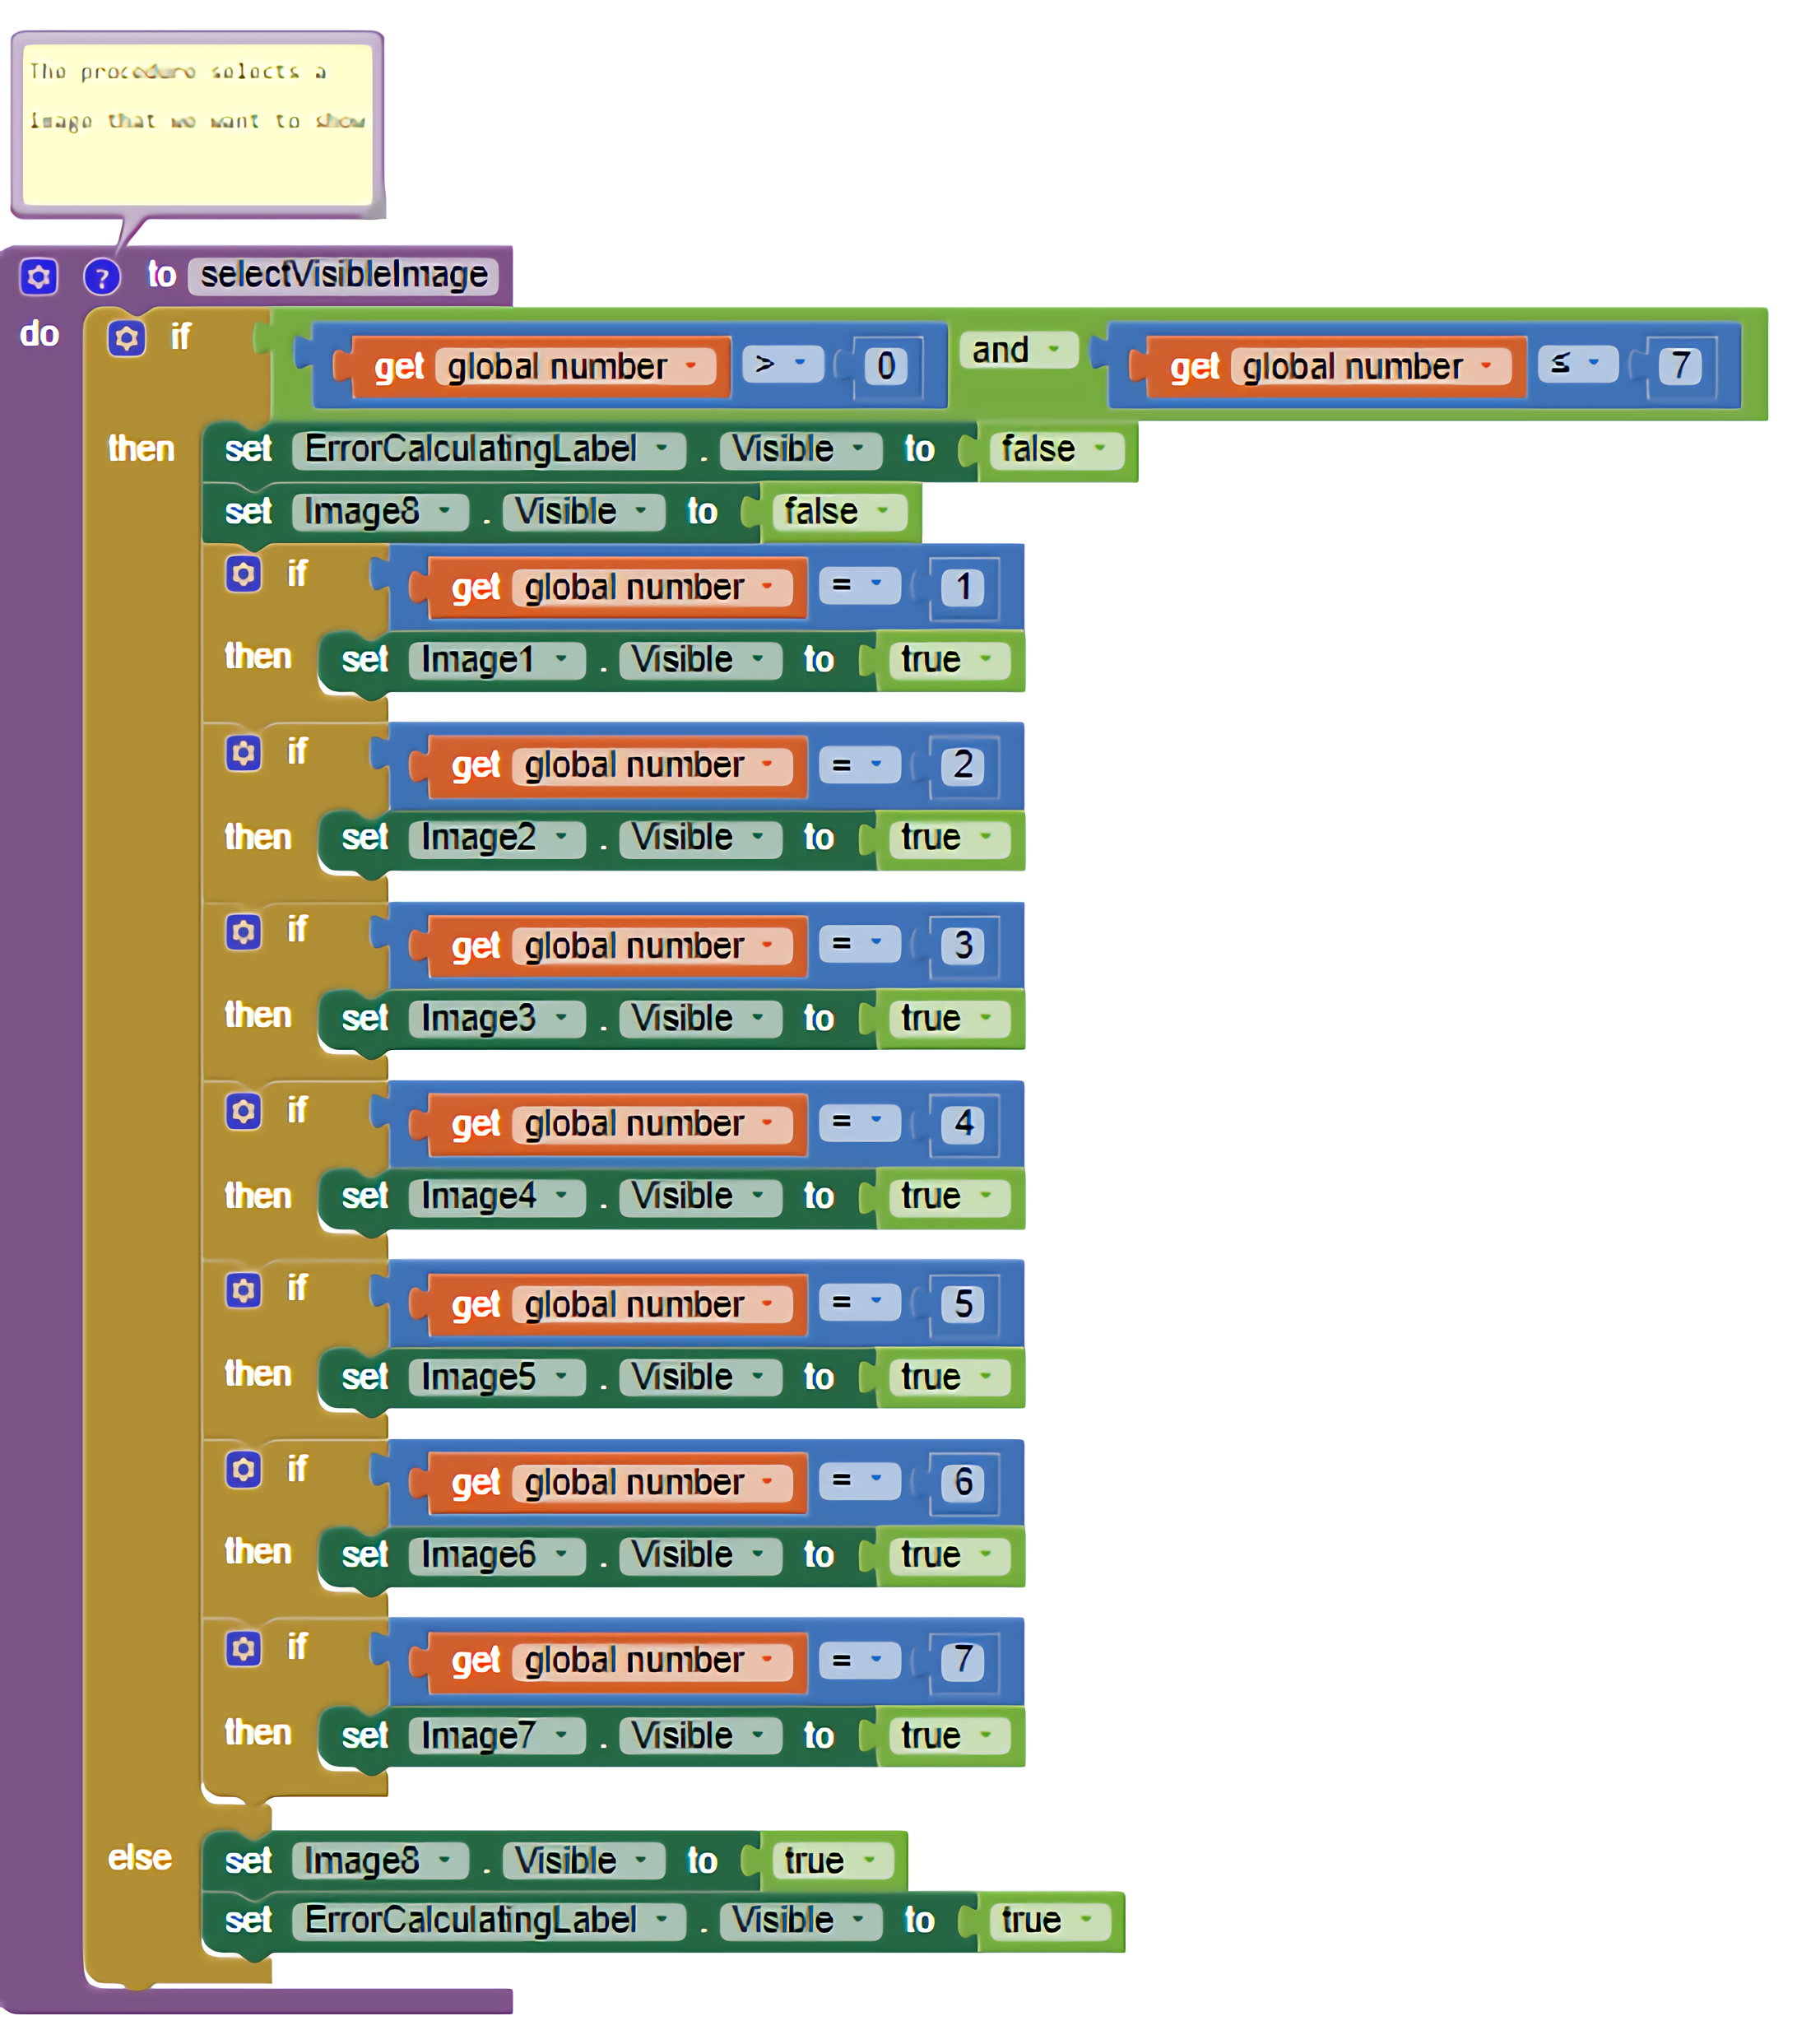
\includegraphics{./graphics/programs/guess_numbers/procedure_selectVisibleImage_AppInventor_2018.png}
    \caption[Процедура selectVisibleImage.][6pt]{Процедура selectVisibleImage управляет отображением изображений с цифрами.}
  \label{fig:block:click:select:visible:image}
\end{figure}

Процедура \textbf{selectVisibleImage} (рис. ~\ref{fig:block:click:select:visible:image}) читает значение глобальной переменной secretNumber и включает рисунок с соответствующей цифрой.
В случае, если число не было определено, показывается изображение с вопросительным знаком (\textit{Image8}).

Например, пусть игрок загадал число три. На основании введённого пользователем числа в поле \textit{numberText} на экране \textit{FinalScreen} (в этом примере должно быть введено число 550) приложение подсчитает и присваивает переменной \textit{secretNumber} новое значение, равное трем. Процедура \textit{selectVisibleImage} в соответствие со значением переменной \textit{secretNumber} делает видимым изображение с соответстующей цифрой. 
В нашем примере это изображение числа три (\textit{Image3}). Если переменная \textit{secretNumber} содержит в себе значение, не входящее в интервал от одного до семи, то будет показано изображение со знаком вопроса (\textit{Image8}), а текст надписи \textit{ErrorСalculating} станет видимым («Допущена ошибка в расчетах. Попробуйте снова.»).

Важно отметить, что перед выполнением условий сравнения переменной \textit{secretNumber} с введенным пользователем числом, выполняется установка свойства \textit{Видимый} (\textit{Visible}) в \textit{false} у элементов Image8 и ErrorСalculating.
Тем самым мы отмечаем отсутствие ошибок в вычислениях и заранее убираем с экрана знак вопроса, предполагая, что на его месте будет изображение с определённой цифрой. Если же переменная secretNumber не входит в интервал от одного до семи, то у элементов \textit{Image8} и \textit{ErrorСalculating} устанавливается значение свойства (\textit{Visible}) в \textit{true}, 
так приложение сообщает пользователю о его ошибке в вычислениях.

\subsection{Работа с экранами}
При проектировании приложения были учтены рекомендации из официальной документации \textit{App Inventor}~\cite{MitManyScreens} по ограничению количества экранов во избежание проблем с переполнением памяти.
Поэтому в игре используется восемь экранов (рекомендуемое количество — меньше 10):
\begin{enumerate}
\item \textbf{Screen1} — главный экран приложения — меню игры.
\item \textbf{About} — экран, содержащий информацию о приложении.
\item \textbf{Step1}, \textbf{Step2}, \textbf{Step3}, \textbf{Step4}, \textbf{Step5} — это экраны с пошаговым описанием задания пользователю. На экранах есть следующие кнопки для навигации между экранами приложения:
\begin{itemize}
  \item \textit{На шаг назад} (\textit{previousStepButton}) меняет экран на предыдущий.
  \item \textit{Далее} (\textit{nextStepButton}) — переход игрока на следующий экран.
  \item \textit{В главное меню} (\textit{backToMainMenuButton}) показывает пользователю главный экран Screen1.
\end{itemize}
\item \textbf{FinalScreen} — это экран с результатами игры. Здесь пользователю необходимо ввести получившееся в результате вычислений число и нажать кнопку «\textit{Узнать ответ}, чтобы увидеть на экране число, которое по предположению программы загадал игрок.
\end{enumerate}

\begin{mdfstyle}[nobreak=true,frametitle=Упражнение]
  \sloppy
  Приложение можно перепроектировать таким образом, чтобы экраны \textit{Step1}, \textit{Step2}, \textit{Step3}, \textit{Step4}, \textit{Step5} представляли собой один экран. Попробуйте реализовать приложение «Угадыватель чисел» с одним общим экраном \textit{Steps}, который будет при нажатии на нём кнопок навигации будет последовательно показывать пользователю пошаговую инструкцию, которые ему необходимо выполнить с загаданным числом.]
  Если вызывать функцию \textit{открыть другой экран} (\textit{open another screen}), а затем не вызывать функцию закрытия экран "\textit{close screen}", то через некоторое время приложение израсходует всю доступную память.
  \end{mdfstyle}

Рассмотрим решение этой проблемы в нашем приложении. Экран \textit{Screen1} содержит в себе элементы интерфейса для отображения название игры и две кнопки: "\textit{Старт}" (\textit{startButton} для перехода на экран \textit{Steps} и "\textit{Об игре}" (\textit{AboutButton} для перехода на экран \textit{About}.

Для того, чтобы не получить ошибку переполнения памяти, создадим процедуру для закрытия экрана, которую назовём \textbf{closeScreen} (рис.~\ref{fig:block:click:close:screen}). Она будет содержать в себе один единственный блок управления "(\textit{close screen}". 
\begin{figure}
  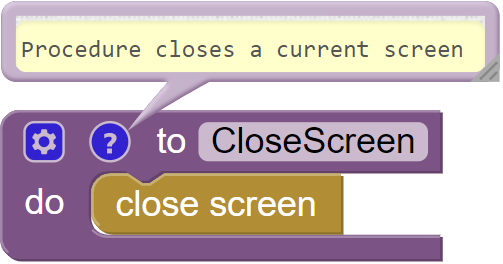
\includegraphics[width=100,height=100]{./graphics/programs/guess_numbers/procedure_closeScreen_AppInventor_2018.png}
    \caption[Процедура closeScreen.][6pt]{Процедура closeScreen закрывает текущий экран.}
  \label{fig:block:click:close:screen}
\end{figure}
Возникает вопрос: зачем действие по закрытию экрана помещать в отдельную процедуру? Это необходимо для того, чтобы последовательно выполнить функции \textit{«open another»} и \textit{«закрыть экран»} при возникновении события нажатия на некоторую кнопку (\textit{Click}). "Пазлы" блоков управления открытия и закрытия так спроектированы, что их нельзя объединить в одном блоке \textit{App Inventor, но можно их разделить через вызов процедуры, что и было сделано (рис.)} Из-за особенностей  соединить функцию закрытия и открытия в любом блоке управления вместе не получится, поэтому способ, описанный выше, решает эту проблему.

